% !TeX TXS-program:compile = txs:///pdflatex/[--shell-escape]
% Le truc au-dessus pour avoir l'option shell-escape qui permet de faire du minted.
\documentclass[11pt]{article}

% Affichage ou non des reponses aux questions & exercices
\newif\ifDispRep
%\DispReptrue  % Show the text
\DispRepfalse % Hide the text

% Version du document
\newcommand{\versiondoc}{v0.1}

% Incorporation tous éléments de préambule communs à tous mes cours
% Sans chemin relatif parce que TexStudio lancé depuis un script qui prend en compte la variable d'environnement TEXINPUTS
\usepackage{CoursLFC}

% Eléments de l'en-tête et de la page de garde spécifiques à ce doc
\newcommand{\classe}{1\textsuperscript{ère} NSI}
\newcommand{\themecours}{"Hors-Série" spécial projets}
\newcommand{\datedoc}{avril 2024}

% Page de garde mise en page
\title
	{\vspace{1cm}
		{\Large
		\textit
			{
				\classe\hspace{0.1cm}
				\textemdash\
				\hspace{0.1cm}
				\themecours
			}
			
		\vspace{1.5cm}
		\huge{Introduction à Pygame}
				 
		\vspace{1cm}
		
		\begin{figure}[H]
			\centering
			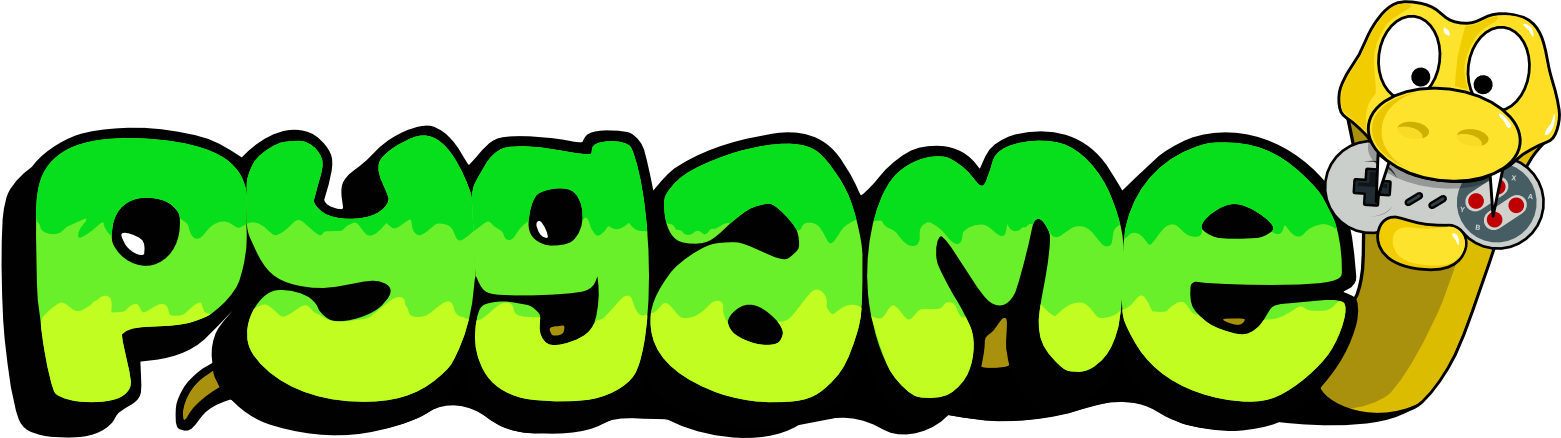
\includegraphics[width=0.6\textwidth]{001_pygame_logo.png}
		\end{figure}
		
		\vspace{1.5cm}
		}
	}
\author{\etablissement}
\date{
	\auteur,
	\datedoc,
	\footnotesize{\textit{\versiondoc}} 
	\vspace{0.5cm}
	}

% Header & Footer
\lfoot{\etabshort}
\cfoot{\thepage}
\rfoot{\classe, \anneescol}
\renewcommand{\footrulewidth}{0.2pt}
\lhead{}
\chead{}
\rhead{}
\renewcommand{\headrulewidth}{0pt}

\begin{document}
	
	\maketitle
	\thispagestyle{empty}
	\vspace{\baselineskip}
	
	\pagebreak
	
	
	\vspace{3cm}
	\tableofcontents
	
	\vspace{5cm}
	\label{ToutVaBien}
	\begin{MonAlarme}{IMPORTANT: pas de panique!}
		Il se peut tout à fait que vous vous retrouviez coincé·e sur ces tâches --- soit parce que vous n'arrivez pas à installer pygame, soit parce que votre environnement Python ne fonctionne pas, soit...
		
		\vspace{\baselineskip}
		C'est tout à fait possible que ça se produise: pas de panique!! Si je suis convaincu que vous avez essayé de résoudre le problème, je ne vous en tiendrai pas rigueur.
		
		\vspace{\baselineskip}
		Je vous demande si ça vous arrive de \uline{\textbf{m'envoyer un mail}} et de vous donner une \uline{vraie} demi-heure d'effort pour résoudre le problème --- et si vous êtes tout de même coincé·e, c'est dommage pour vous mais ça peut arriver... Prévenez-moi et on verra à la rentrée si je n'ai pas le temps de vous répondre pendant les vacances.
		
		\vspace{\baselineskip}
		En tout état de cause: bonnes vacances à tous!
		
	\end{MonAlarme}
	
	% pas de footer sur la première page
	\thispagestyle{empty}
	\vspace{\baselineskip}
	
	\pagebreak
	
	
	% Début du contenu du document
	\section{Introduction \& pré-requis}
	\subsection*{Introduction}
	Le but de ce document est de vous guider pas à pas dans la découverte du module Pygame. Il n'est pas à proprement parler un cours --- d'ailleurs il n'est pas au programme en tant que tel. C'est un guide pour vous permettre de faire des choses en Python, dans le cadre de vos projets notamment, un peu plus "marrantes" que ce que l'on fait dans le cadre de nos exercices de cours.
	
	\begin{MonAmp}{Comment utiliser ce document}
		\begin{itemize}
			\item J'ai essayé de rendre ce document complet pour que vous ne vous retrouviez pas coincés --- mais du coup il est long. Mon conseil: ne regardez que le code et les activités pour commencer:
			\begin{itemize}
				\item Copiez / collez les programmes Python, exécutez-les, et essayez de comprendre par vous-même comment ils fonctionnent;
				\item Modifiez-les ensuite selon les instructions dans les activités proposées (encadrés verts).
				\item \textit{Et si quelque chose vous échappe, cherchez dans le reste du texte de ce document -- ce sera sûrement expliqué!}
			\end{itemize}
			\item J'utilise le verbe "bidouiller" à plusieurs reprises dans ce document --- et c'est \textbf{\textit{vraiment}} ce que je veux que vous fassiez: changez une valeur dans votre code, exécutez-le pour voir ce que ça donne; recommencez avec une autre valeur; puis avec une autre... Il n'y a strictement aucun risque à faire ça (dans le pire des cas ça vous donnera une erreur -- et alors?!?) et c'est comme ça que vous verrez ce que fait le code et que vous apprendrez.
			\item Dernier point: tout le code que j'ai inclus dans ce document est \href{https://www.dropbox.com/scl/fi/ssngjj5nxguwcrr563pge/_code.zip?rlkey=zgrmhxhbaz5wi50m6whphosb8&dl=0}{téléchargeable ici} --- ça vous évitera de devoir faire des copier / coller de ce document (et de devoir supprimer les numéros de ligne)...
		\end{itemize}
	\end{MonAmp}
	
	J'ai essayé d'être le plus complet possible ici pour éviter que vous ne risquiez de vous retrouver bloqués --- et du coup, ce document est assez long. Si vous êtes à l'aise n'hésitez pas à sauter des sections pour avancer plus vite!
	
	\subsection*{Avant de commencer --- pré-requis}
	Pour pouvoir effectuer les tâches listées dans ce document (et plus généralement utiliser Pygame), il y a plusieurs solutions:
	\begin{itemize}
		\item L'idéal est d'être sur une machine pour laquelle vous avez accès au compte administrateur (c'est a priori le cas de n'importe quel ordinateur appartenant à votre famille si vous en avez un; \textbf{ce n'est en revanche pas le cas des machines "Région île de France"} (voir ci-dessous pour celles-là)):
		\begin{itemize}
			\item Vérifiez que Python est installé sur la machine --- lancez l'application IDLE. Si elle s'ouvre, c'est bon. Si ce n'est pas le cas et que vous êtes sous Windows suivez les instructions listées sur \href{https://docs.python.org/fr/3/using/windows.html#windows-full}{cette page}.
			\item Choisissez l'environnement dans lequel vous allez taper votre code --- ça peut être IDLE, Visual Studio Code, EduPython (si vous ne savez pas décider je vous conseille EduPython): ouvrez-le.
			\item Vérifiez que pygame est installé dans cet environnement: tapez \texttt{import pygame} dans un script et exécutez-le. 
			\begin{itemize}
				\item Si il passe à la ligne suivante sans afficher de message (ou vous affiche un petit message de bienvenue), c'est bon --- vous pouvez aller directement à la section 4 de ce document pour commencer les activités.
				\item Si il vous affiche ceci (et il y a des chances que ce soit le cas), il faudra installer pygame.
				
				\begin{figure}[H]
					\centering
					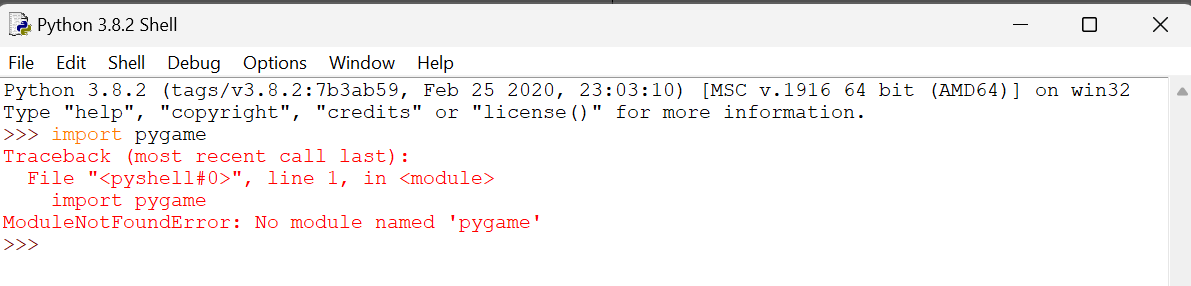
\includegraphics[width=0.8\textwidth]{002_pygame_not_installed.png}
				\end{figure}
				Pour installer pygame (sous Windows):
				\begin{itemize}
					\item Ouvrez une ligne de commande: appuyez simultanément sur les touches Windows et R (\faWindows \quad+\quad R) puis tapez "cmd" et Entrée ($\hookleftarrow$).
					\item Tapez la commande: \texttt{pip install pygame}.
					\item Quelque chose comme l'image ci-dessous va s'afficher; patientez (ça peut durer une à deux minutes) jusqu'à ce que ce soit terminé, et ce sera bon --- vous pourrez passer à la section 4 de ce document pour commencer les activités.
					
					\begin{figure}[H]
						\centering
						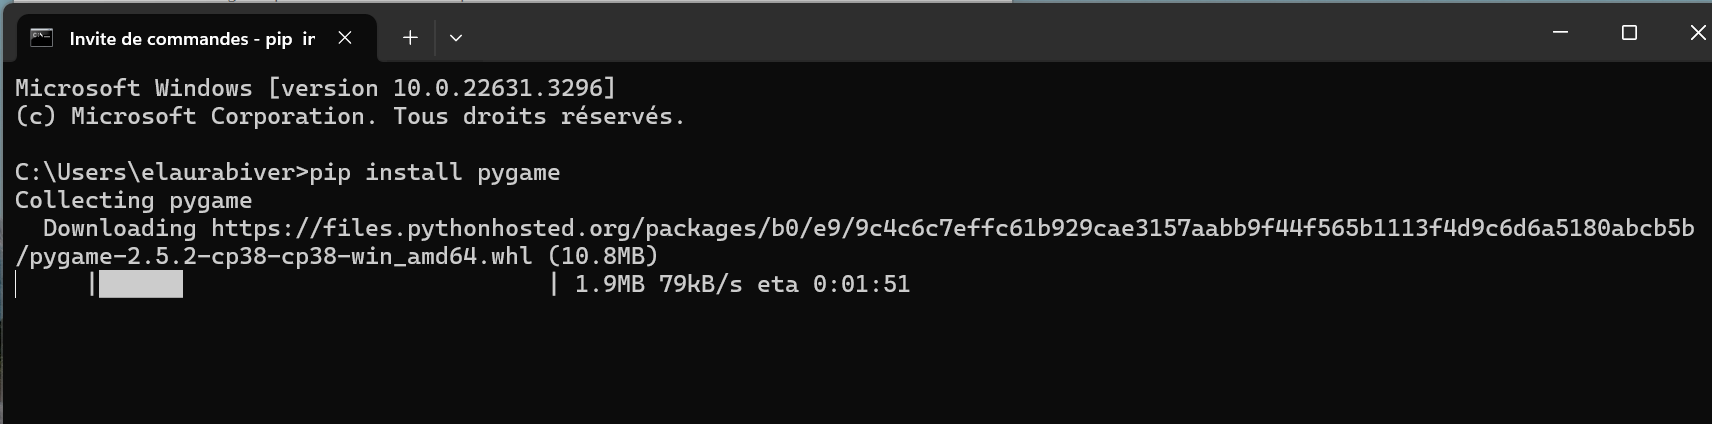
\includegraphics[width=0.8\textwidth]{003_pygame_install.png}
					\end{figure}
				\end{itemize}
			\end{itemize}
		\end{itemize}
		\item Si vous n'avez pas d'autre choix que d'utiliser votre ordinateur de la Région île de France (soit parce que vous n'avez pas d'autre machine soit parce que vous n'avez pas réussi à installer Python ou pygame), vous allez devoir utiliser EduPython pour lequel pygame est déjà installé\footnote{Vous ne pouvez pas utiliser IDLE parce qu'il pointe vers un environnement où pygame n'est pas installé et vous n'avez pas les droits administrateur pour l'installer}.
		\begin{figure}[H]
			\centering
			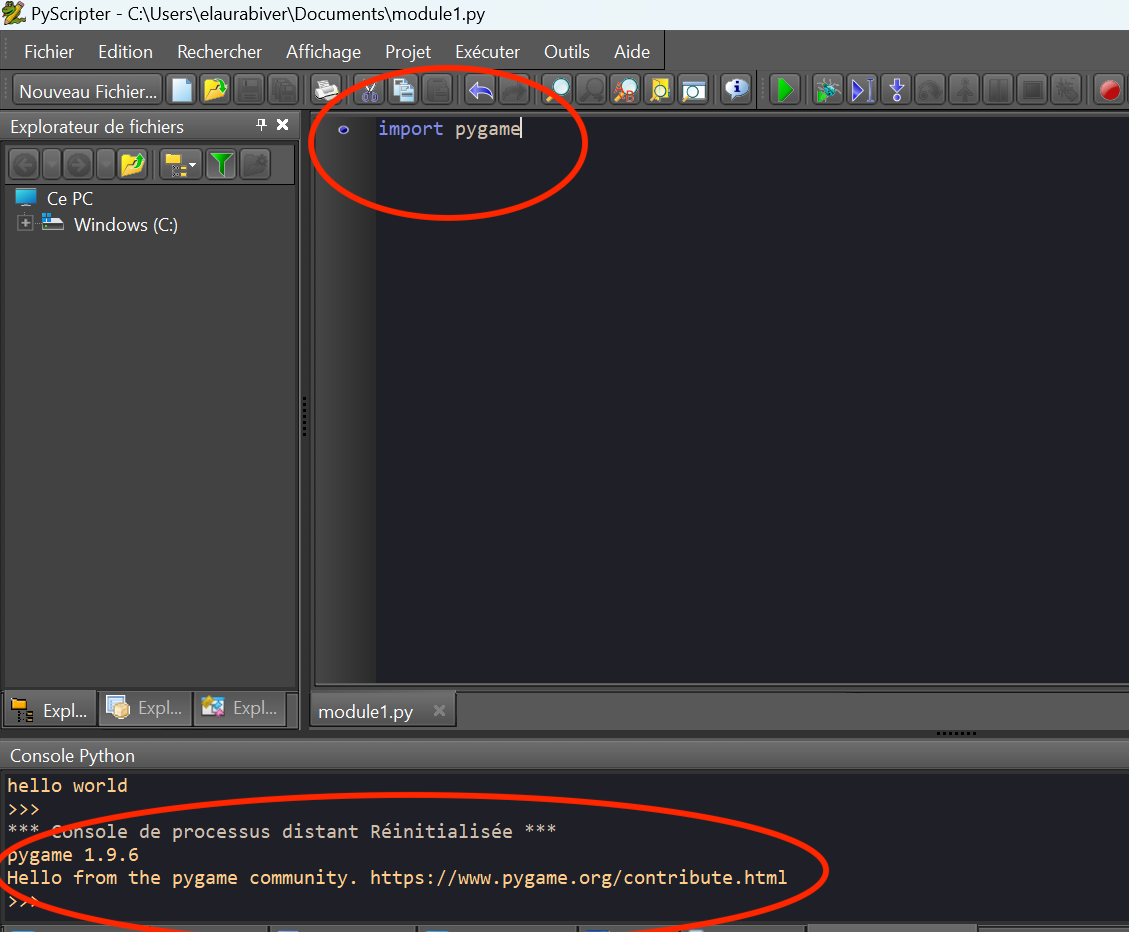
\includegraphics[width=0.6\textwidth]{004_pygame_edupython.png}
		\end{figure}
	\end{itemize}
		
	\section{Si ce document ne nous plaît pas, on fait quoi?}
	J'essaye de vous faire découvrir pygame et plus généralement la programmation qu'on appelle "événementielle" dans Python dans ce document. Mais il y a une foule immense d'autres sources possibles en ligne --- et ce serait idiot de vous restreindre à ce document-ci si il ne vous convient pas. Alors si vous voulez aller chercher un peu plus loin, voici des pistes que je vous propose:
	\begin{itemize}
		\item Avant tout: \textbf{n'oubliez pas d'utiliser \href{https://chat.openai.com}{ChatGPT}}!! Si vous écrivez du code mais qu'il ne marche pas, donnez-le à ChatGPT et demandez-lui ce qui ne va pas; si votre code ne fait pas ce que vous voulez, copiez-le aussi, décrivez ce que vous voudriez qu'il fasse, et demandez-lui ce qui ne va pas; etc....
		\item N'hésitez pas à consulter \href{https://www.pygame.org/docs/}{la documentation officielle du module Pygame} (en français ici, mais elle existe dans de nombreuses autres langues).
		\item Pour ce document je me suis beaucoup inspiré de \href{https://nsimeyroneinc.github.io/NSI1_2022_2023/T08_Extras/3Pygame/01-Pygame_intro/}{ce site} --- n'hésitez pas à le consulter!
		\item \href{https://www.zonensi.fr/Miscellanees/Pygame/Base_pygame/#creation-dune-fenetre-graphique-et-boucle-devenements}{Un cours pour les spécialité NSI spécialement orienté pygame}.
		\item Le site \href{https://jeux.developpez.com/tutoriels/Pygame/}{developpez.com} propose différents cours concernant Pygame. Ils ne me semblent pas très parlants, mais jettez-y un coup d'\oe{}il quand même --- peut-être qu'ils vous conviendront!
		\item Il existe également beaucoup de ressources en video:
		\begin{itemize}
			\item La meilleure de toutes me semble être \href{https://www.youtube.com/watch?v=xxRhvyZXd8I&list=PLX5fBCkxJmm1fPSqgn9gyR3qih8yYLvMj}{celle-ci} --- mais elle est malheureusement en anglais.
			\item \href{https://www.youtube.com/watch?v=E1P6N5ZplWk&list=PL_Jc8T8naBEUuc0t-nGg9tuhwGfMUqz2H}{Une introduction à pygame} --- moins bien faite que celle ci-dessus je pense, mais elle est en français.
		\end{itemize}
		\item \textbf{Et si vous voulez aller plus loin, \href{https://realpython.com/platformer-python-arcade/}{ce site} vous propose tout un tas de ressources (tuiles de fond, personnages, musiques...) gratuitement!}
	\end{itemize}
	Je m'arrête là --- mais n'hésitez pas à chercher par vous-mêmes!
	
	\section{Une fenêtre sans mouvement}
	\subsection*{Notre première fenêtre Pygame: juste un fond}
	Dans votre environnement de développement choisi, entrez le code suivant, enregistrez-le (donnez-lui par exemple le nom "pygame-etape01.py"), et exécutez-le:
	\vspace{0.1cm}
	\MonPython{Pygame_001_Intro.py}
	
	Explication(s) de texte:
	\begin{description}
		\item[Lignes 2 \& 3:] Ici, on importe le module Pygame ainsi que des variables locales bien utiles pour la suite. Ces deux lignes sont à systématiquement intégrer dans tout programme s'appuyant sur Pygame.
		\item[Ligne 9:] On définit la fenêtre que l'on va ouvrir -- ses dimensions, ici, vont être 640 pixels de large par 480 pixels de haut.
		\item[Ligne 10:] On définit la couleur de fond de notre fenêtre: ici on a choisi (en code RGB ("Red / Green / Blue") une nuance de turquoise (si vous voulez vous amuser à tester d'autres couleurs, \href{https://www.rapidtables.com/web/color/RGB_Color.html}{ce site} vous permettra de le faire aisément).
		\item[Ligne 13: ] Cette commande effectue un rafraîchissement total de tous les éléments graphiques de la fenêtre --- on ne le fait qu'une fois ici puisqu'on n'a qu'une fenêtre vide, mais quand on aura des animations ce sera fait très régulièrement...
		\item[Ligne 17:] Les jeux fonctionnent souvent ainsi: on crée une boucle "infinie" dans laquelle tous les événements du jeu vont se succéder et on n'en sort qu'à la fin du jeu qui est provoquée par la bascule d'un booléen --- ici \texttt{continuer}.
		\item[Ligne 18:] Tout au long de cette boucle infinie, on va gérer des "événements" que pygame nous renvoie par la fonction \texttt{pygame.event.get()} --- on reviendra sur cette notion dans la section 5 de ce document.
		\item[Lignes19 \& 20:] Les événements peuvent être classés par type: ici on va se limiter au type \texttt{QUIT} qui correspond à une fermeture de la fenêtre (par un clic sur la croix en haut à droite par exemple, sous Windows). Dans ce cas on positionne \texttt{continuer} à \texttt{False} et donc on sort de la boucle pour conclure (ligne 23) par une sortie propre avec \texttt{pygame.quit()}.
	\end{description}
	
	\begin{MonAct}[bidouillons cette première fenêtre!]
		Pour vous familiariser un peu avec ce nouvel environnement, faites des modifications dans le code précédent et exécutez-le pour en voir les effets: modifiez la couleur de fond -- passez-là par exemple en noir, en blanc, en bleu; modifiez les dimensions de la fenêtre.
		
		Le but dans ces activités "bidouillons" est vraiment que vous n'hésitiez pas à essayer différentes valeurs pour bien vous rendre compte du fonctionnement du module pygame.
	\end{MonAct}
	
	\subsection*{Ajoutons un ballon de foot}
	Pour cette prochaine étape, nous allons importer une image et la mettre dans notre fenêtre pygame --- toujours sans animation pour le moment:
	\begin{itemize}
		\item Commencez pas télécharger \href{https://github.com/marc-biver/Vrac/blob/main/ballon.png}{le fichier \texttt{ballon.png} que nous allons utiliser en cliquant sur ce lien}.
		\item Placez ce fichier \texttt{ballon.png} dans le même répertoire que celui où vous enregistrez vos scripts Python.
	\end{itemize}
	
	Maintenant qu'on a cette image, on va chercher à la placer dans notre fenêtre pygame. Ca se fait de manière assez simple, à un détail près: les coordonnées partent du coin en haut à gauche de la fenêtre au lieu de partir d'en bas à gauche comme on a l'habitude. Le repère qu'on utilise a donc cette tête (avec l'origine dans le coin en haut à gauche de la fenêtre):
	
	\begin{figure}[H]
		\centering
		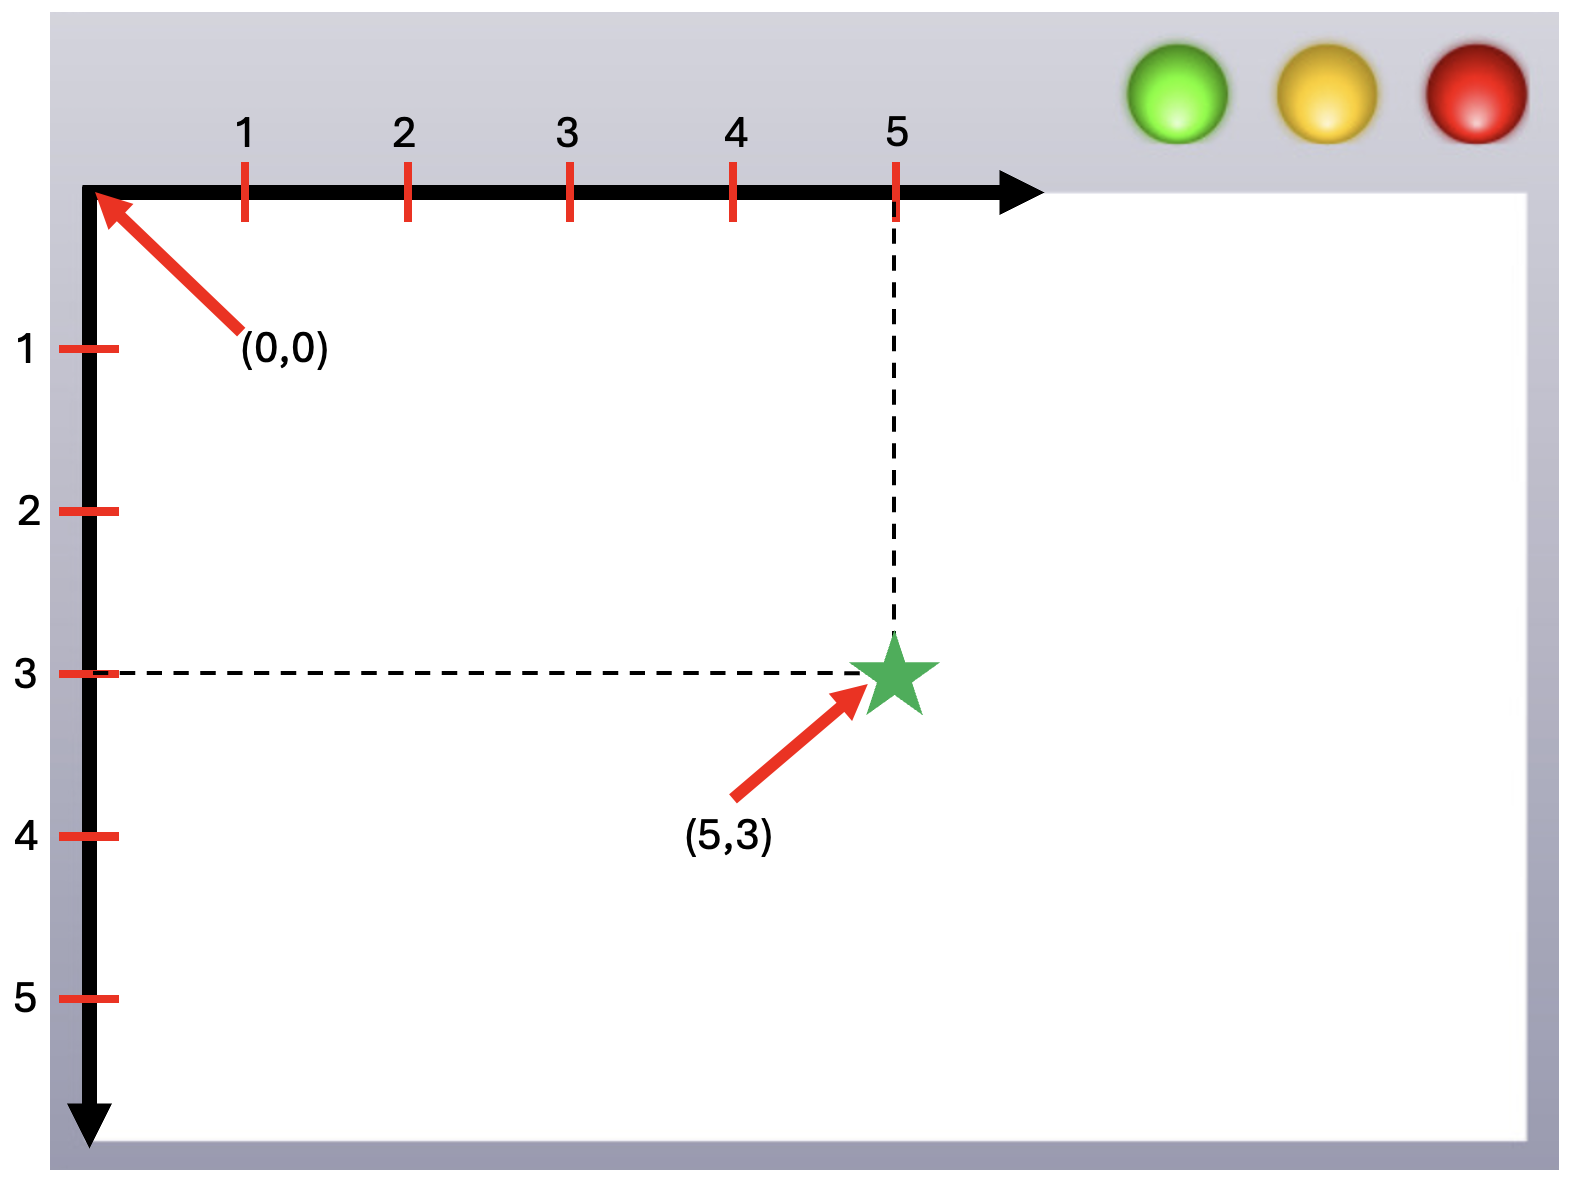
\includegraphics[width=0.6\textwidth]{005_pygame_repere_ortho.png}
	\end{figure}
	
	Dans votre environnement de développement choisi, entrez le code suivant, enregistrez-le (donnez-lui un nom qui fait suite au précédent, par exemple "pygame-etape02.py), et exécutez-le:
	\vspace{0.1cm}
	\MonPython{Pygame_002_Balle.py}
	
	Explication(s) de texte:
	\begin{description}
		\item[Lignes 10 \& 11:] Ici, on "charge" l'image du ballon (fonction \texttt{load}) --- on dit à Python de la prendre en compte et d'être prêt à l'afficher sous le nom qu'on lui a donné, ici "\texttt{balle}". On redimensionne l'image également (fonction \texttt{scale}, ce qui signifie "échelle") à 60 pixels par 60 pixels, pour qu'elle tienne bien dans notre fenêtre.
		\item[Lignes 14 \& 15:] On place la balle dans la fenêtre. Dans un premier temps on définit sa position (dans le repère décrit ci-dessus) et on la dessine (en utilisant la fonction \texttt{blit}).
		\item[Lignes qui suivent:] Rien de plus que dans le code précédent...
	\end{description}
	
	\begin{MonAct}[et si on déplaçait ce ballon un peu?]
		Essayez, en jouant sur les coordonnées entrées dans la ligne 14 du code, de déplacer le ballon pour le mettre dans le coin tout en haut à gauche, puis tout en haut à droite, puis tout en bas à gauche, puis tout en bas à droite.
		
		Qu'est-ce que vous concluez sur la signification de ces coordonnées? Est-ce qu'elles correspondent à où vous placez le centre du ballon, ou autre chose? (N'oubliez-pas qu'on a dimensionné le ballon pour qu'il fasse $60 \times 60$ pixels).
	\end{MonAct}
	
	\section{Et si on le lançait, ce ballon?}
	Là, on rentre dans une dimension totalement différente --- il ne s'agit plus de représenter une image dans une fenêtre mais de la faire bouger et de prévoir \textit{comment} elle va bouger. Ca va vous demander des compétences en informatique, mais aussi en maths et un peu en physique....
	
	La première notion à comprendre est celle de "Frame Per Second" (FPS), que l'on peut traduire par "image par seconde": comme au cinéma, un écran pygame est une succession d'images que votre programme va dessiner les unes après les autres, à un rythme déterminé en FPS\footnote{En général, on considère qu'à partir de 24 images par seconde l'oeil humain est incapable de voir les images individuellement --- et a donc l'impression de voir un film si elles s'enchaînent bien.}. A partir du moment où les images s'enchaînent logiquement et suffisamment vite l'oeil humain aura l'impression d'un mouvement: par exemple, les images ci-dessous pourraient, si on en avait beaucoup plus et qu'on les faisait défiler très rapidement, donner l'impression que le ballon se déplace de gauche à droite.
	
	\noindent % Prevent indentation
	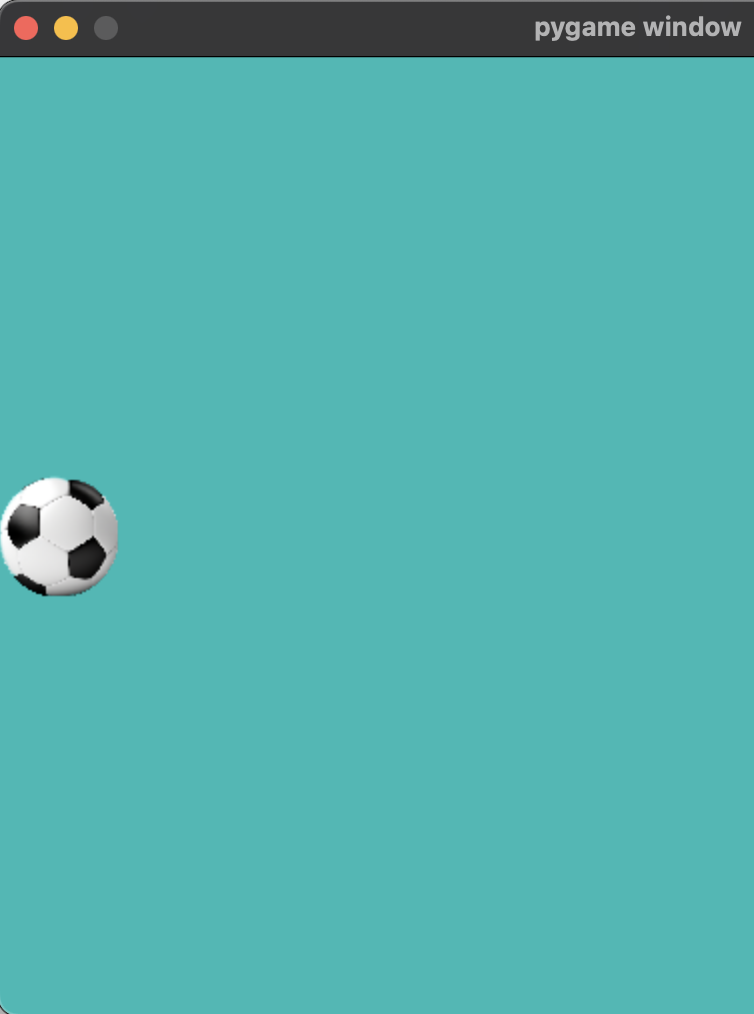
\includegraphics[width=0.18\textwidth]{006_Ball_P1.png}
	\hfill
	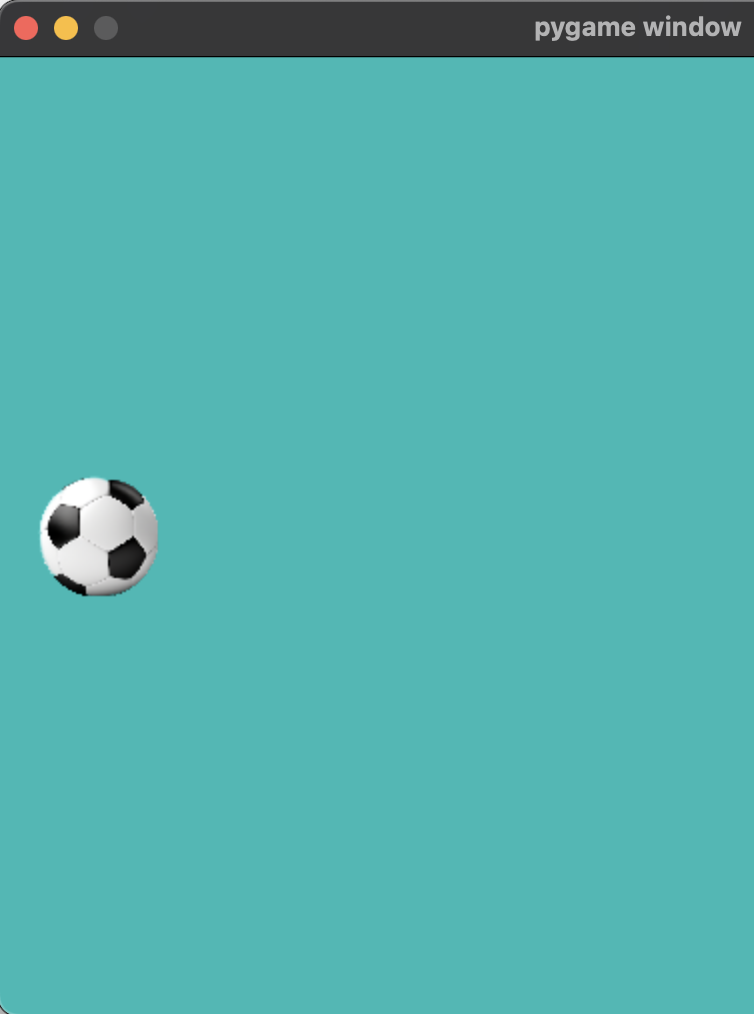
\includegraphics[width=0.18\textwidth]{007_Ball_P2.png}
	\hfill
	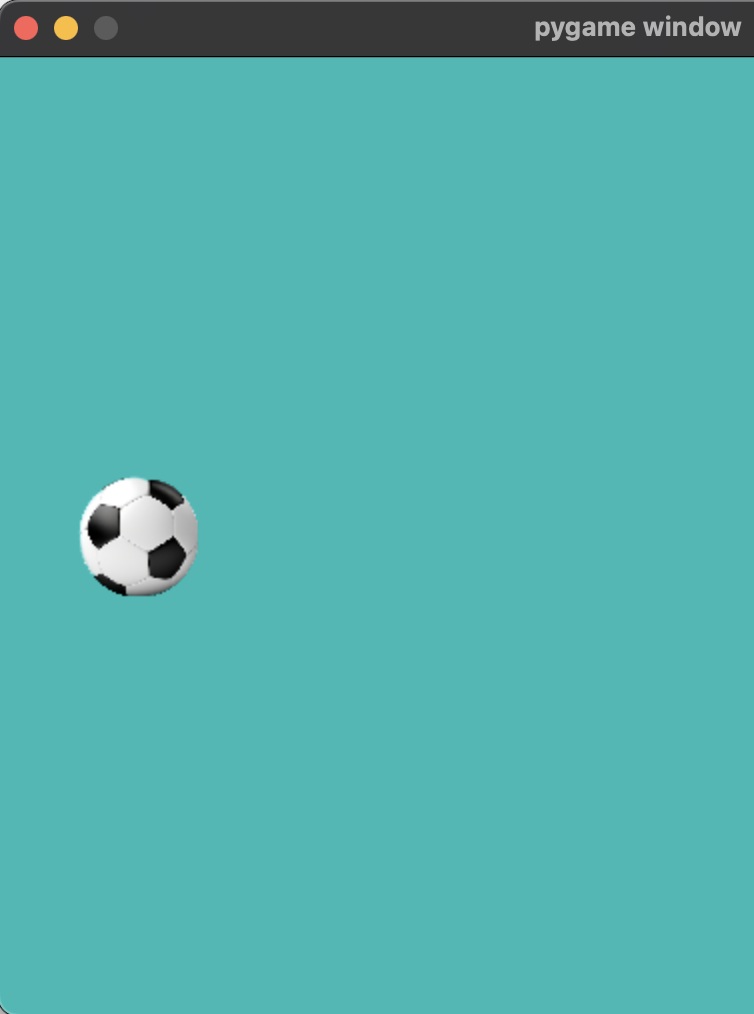
\includegraphics[width=0.18\textwidth]{008_Ball_P3.png}
	\hfill
	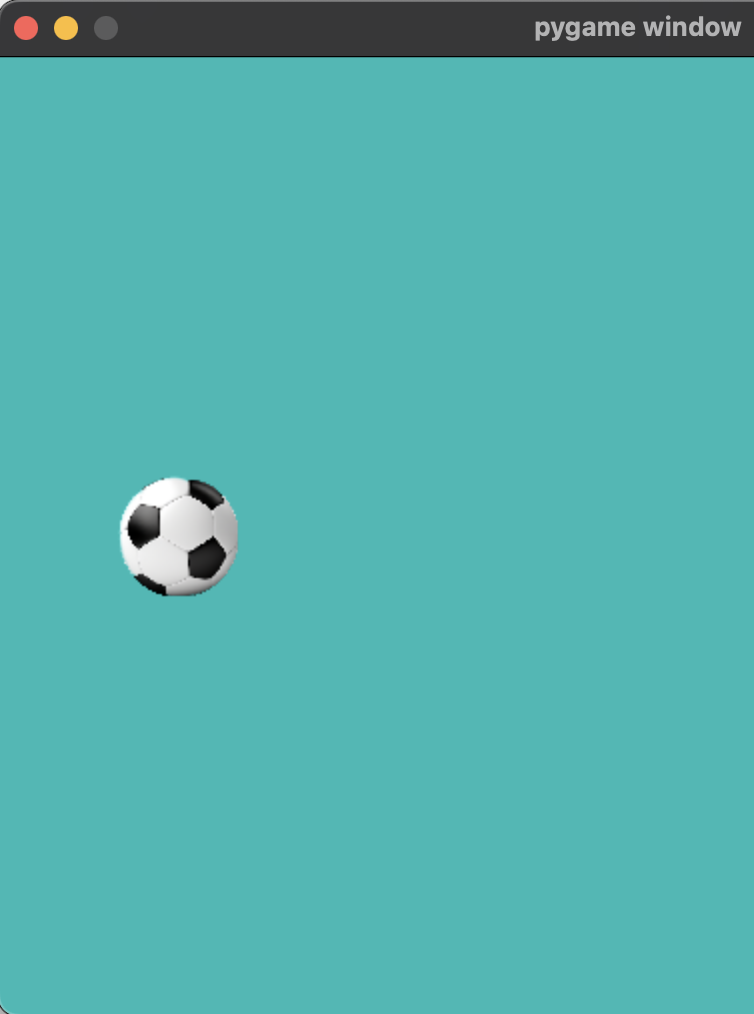
\includegraphics[width=0.18\textwidth]{009_Ball_P4.png}
	\hfill
	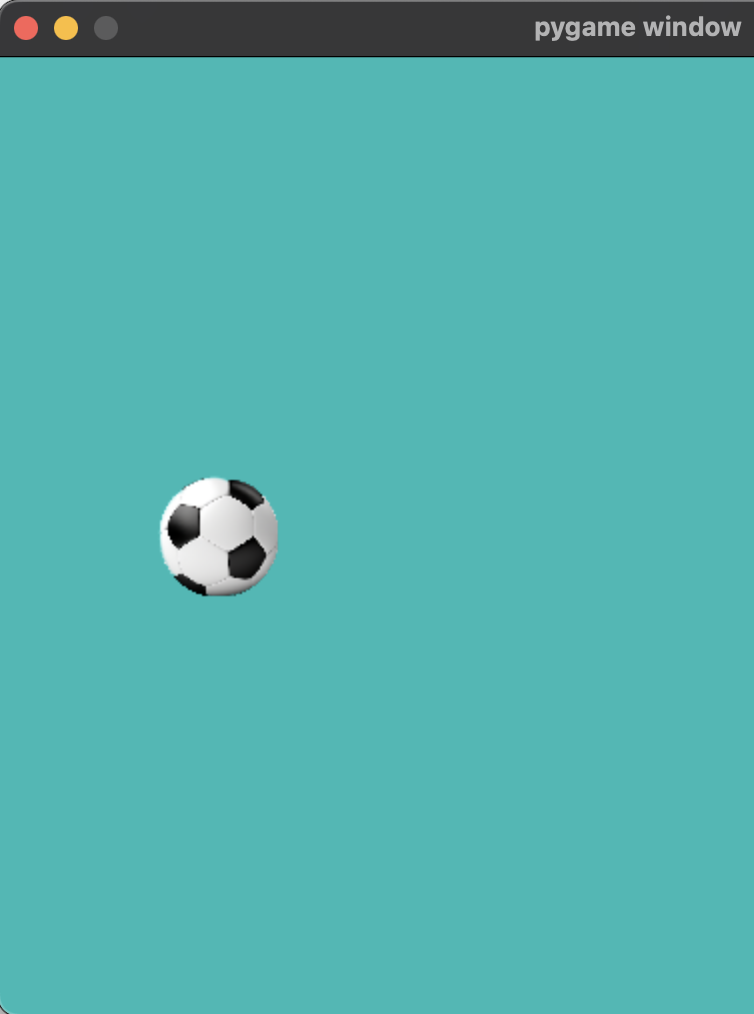
\includegraphics[width=0.18\textwidth]{010_Ball_P5.png}
	
	\subsection*{Dans une pièce sans murs...}
	Commençons par faire ce que les images ci-dessus commençaient à faire: lançons le ballon simplement du bord gauche vers la droite:
	
	\MonPython{Pygame_003_Lancer.py}
	
	Explication(s) de texte:
	\begin{description}
		\item[Lignes 11 \& 35:] Ces deux lignes sont là pour que pygame régule la vitesse d'exéxution du programme à un FPS constant: ici, 60.
		\item[Ligne 27:] "Lancer" le ballon de la gauche vers la droite revient à augmenter progressivement son abscisse. Ici, on l'augmente de 5 pixels à chaque tour de boucle, donc de $60 \times 5 = 300$ pixels par seconde (puisqu'on est à 60 FPS).
		\item[Ligne 31:] Une fois qu'on a défini la nouvelle position du ballon, il nous reste à le dessiner de nouveau au moyen de la fonction \texttt{blit} comme précédemment.
	\end{description}
	
	\begin{MonAct}[effacer la trainée]
		Normalement, si vous avez exécuté le code ci-dessus, vous avez du voir que le ballon ne se déplaçait pas vraiment --- on dirait plus qu'il s'étale sur l'écran, non? La raison est simple: votre boucle, à chaque tour, dessine le ballon à sa nouvelle position, mais sans effacer la position précédente --- et donc le dessin de la position précédente reste. Comment faire pour éviter ça? Corrigez le code pour que le ballon se déplace proprement\footnote{Si vous avez besoin d'un indice: la solution consiste à redessiner à chaque fois la fenêtre vide avant de dessiner la nouvelle position du ballon --- et pour faire ça on utilise tout simplement la fonction \texttt{fill}.}.
	\end{MonAct}
	
	Remarque: vous noterez que le ballon finit par complètement quitter la fenêtre. C'est normal: une fois que l'abscisse de la position du ballon a dépassé la largeur de la fenêtre (1500 dans ce cas), alors on ne voit plus le ballon!
	
	\begin{MonAct}[bidouillons ce lancer de balle...]
		N'hésitez pas à exécuter ce code plusieurs fois en faisant varier la vitesse (le "\texttt{+= 5}"), mais aussi le FPS (le 60 dans "\texttt{clock.tick(60)}"), la position de départ, les dimensions de la fenêtre...
		
		Essayez de faire évoluer aussi l'ordonnée (donc \texttt{balle\_y}) pour modifier la direction du lancer!
	\end{MonAct}
	
	\subsection*{Et si on lui met un mur en face?}
	On va ici chercher à faire rebondir le ballon: s'il arrive à une vitesse $v$ contre le bord droit de la fenêtre (qu'on va imaginer être un mur), on voudrait qu'il rebondisse dessus et reparte à la vitesse $v$ dans l'autre sens.
	
	Pour cela on va utiliser une autre notion, la seule qui est (éventuellement) un peu difficile dans pygame --- celle de "rectangle". Quand vous vous voyez un personnage, ou un arbre, ou n'importe quelle autre représentation dans votre jeu, pygame, lui, voit un rectangle qui l'entoure au plus près. Et c'est ce rectangle que pygame utilise pour positionner votre objet, gérer ses éventuelles collisions (contre d'autres objets par exemple), etc...
	
	Donc quand vous voyez \raisebox{-0.5\height}{
\includegraphics[height=2em]{011_Ballon.png}} pygame est en fait en train de gérer \raisebox{-0.5\height}{
\includegraphics[height=2em]{012_Rect.png}}.
	
	Un autre exemple: dans un jeu de combat très basique où pour faire perdre des points de vie à votre adversaire il faut lui donner un coup de poing dans la tête, vous pourrez voir quelque chose comme ceci \raisebox{-0.5\height}{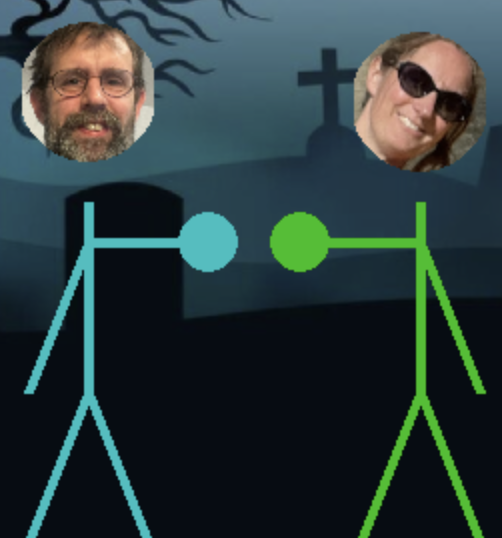
\includegraphics[height=6em]{013_DoomFighter.png}} alors qu'en fait pygame, lui, analyse les collisions (coups) entre poing et tête en gérant ces formes beaucoup plus simples: \raisebox{-0.5\height}{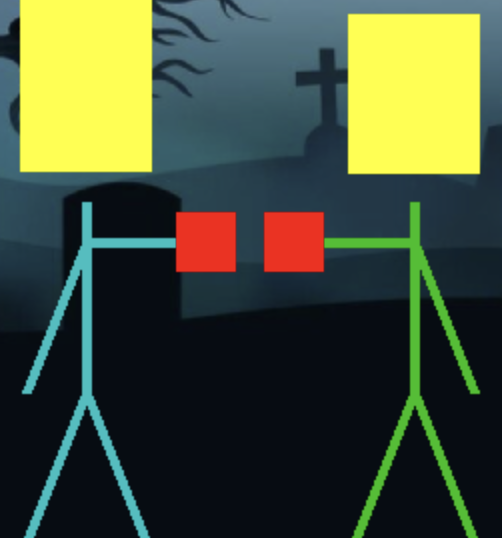
\includegraphics[height=6em]{014_DoomRect.png}} (et il considèrera qu'un coup a été donné quand un des rectangles rouge se superpose à un rectangle jaune).
	
	Ce que l'on va faire à partir de maintenant, c'est manipuler ces rectangles à la place des objets eux-mêmes, et ensuite tout simplement placer l'objet sur son rectangle. L'intérêt? Par exemple on peut directement utiliser une fonction "move" sur un rectangle à laquelle on passe en argument un vecteur vitesse --- plutôt que de recalculer les nouvelles coordonnées à chaque fois comme on l'a fait à l'étape précédente. 
	
	D'ailleurs voici un programme qui fait \textit{exactement}\footnote{\textit{Presqu'}exactement en fait: cette version efface la trace du ballon quand il se déplace.} la même chose que le précédent mais avec une gestion par rectangles:
	
	\MonPython{Pygame_004_LancerRect.py}
	
	Explication(s) de texte:
	\begin{description}
		\item[Enchaînement lignes 11, 12, 15, et 16:] Ces quatre lignes vont ensemble et si vous les comprenez vous aurez tout compris aux rectangles:
		\begin{itemize}
			\item \textbf{Lignes 11 et 12:} je charge et je redimensionne l'image, comme précédemment --- \textbf{\textit{et pour l'instant je n'ai rien affiché}}: l'image est juste en mémoire, aux bonnes dimensions;
			\item \textbf{Ligne 15:} je récupère le rectangle de la balle: pygame me le dimensionne (sur la base de la taille de la balle) et moi (le développeur) je le positionne ("\texttt{topleft = (0, 210)}");
			\item \textbf{Ligne 16:} l'image est chargée, le rectangle est en place --- il me reste juste à dessiner l'image dans la fenêtre, à la position du rectangle.
		\end{itemize}
		\item[Ligne 28:] J'utilise directement la fonction "move" à la vitesse que j'ai définie --- et pygame me déplace mon rectangle comme j'en ai besoin;
		\item[Ligne 34:] Tout ce que j'ai à faire c'est, à chaque passage dans la boucle, dessiner la balle à l'endroit où se trouve son rectangle.
	\end{description}
	
	Et ceci va nous permettre très simplement de gérer le rebond contre les murs:
	
	\MonPython{Pygame_005_Rebond.py}
	
	Explication(s) de texte:
	\begin{description}
		\item[Lignes 32 \& 33:] C'est la seule nouveauté par rapport au code précédent: on vérifie si le côté droit de la balle atteint le bord droit de la fenêtre ou si le côté gauche de la balle atteint son côté gauche et si c'est le cas on inverse la composante $x$ de la vitesse (\texttt{vitesse[0]}) et donc le ballon repart dans l'autre sens (puisque pour le moment il ne se déplace qu'horizontalement).
	\end{description}

	\begin{MonAct}[et si on ne lance pas le ballon horizontalement?]
		Imaginons qu'on n'envoie plus le ballon horizontalement, mais en diagonale à la place? Voici les éléments à prendre en compte / quelques indices:
		\begin{itemize}
			\item Un vecteur vitesse diagonal sera de type \texttt{[$n$, $n$]} --- commencez par exemple avec \texttt{[5, 5]};
			\item Un rebond sur le bord droit ou le bord gauche inversera la vitesse horizontale, donc sa composante en abscisse, donc \texttt{vitesse[0]};
			\item Un rebond sur le bord haut ou le bord bas inversera la vitesse verticale, donc sa composante en ordonnée, donc \texttt{vitesse[1]};
			\item Notez que, dans le code, les dimensions de la fenêtre sont stockées dans des variables (\texttt{Largeur\_Fenetre} et \texttt{Hauteur\_Fenetre});
			\item N'oubliez pas que l'ordonnée 0 est celle du haut de la fenêtre que celle du bas, du coup, est \texttt{Hauteur\_Fenetre};
			\item Et je vous donne enfin quatre propriétés utiles des objets de tyme \texttt{rect}: \texttt{ballrect.top, ballrect.bottom, ballrect.left, ballrect.right} qui ont respectivement les valeurs de l'ordonnée du haut du rectangle, celle de son bas, l'abscisse de la gauche du rectangle et enfin celle de sa droite.
		\end{itemize}
		
		Je vous donne ci-dessous le corrigé de cette activité --- mais \uline{\textbf{je vous encourage vivement à essayer de la réaliser vous-même}}. Vous verrez, elle est en fait assez simple!
	\end{MonAct}
	
	Comme promis, donc, le code de la balle lancée en diagonale avec ses rebonds sur les bords:
	\label{RebondDiag}
	\MonPython{Pygame_006_Diagonale.py}
	
	\section{Et si, maintenant, on le contrôlait, ce ballon?}
	Jusqu'ici on a programmé un petit film, celui d'un ballon en mouvement perpétuel, mais on ne peut pas vraiment dire qu'on a programmé un jeu --- le ballon, on peut le regarder, mais sans toucher au code du programme, on ne peut pas le contrôler. Pour pouvoir gérer ça, on va faire ce que l'on appelle de la programmation "événementielle", c'est-à-dire qui réagit à des actions effectuées par l'utilisateur que l'on va appeler des événements. Ces événements, qu'on a un tout petit peu évoqué au début de ce document avec le type "\texttt{QUIT}" peuvent en réalité être de multiples natures: des touches sur lesquelles on tape, des mouvements ou des clics de souris, voire, pour les écrans tactiles, des gestes de doigts sur l'écran. Tout événement qui n'est pas explicitement listé n'aura aucun impact --- par exemple, sur tous les programmes qu'on a faits jusqu'à présent, si vous tapez sur une touche du clavier, rien ne se produira puisque le cas n'est pas prévu dans le programme.
	
	Commençons par un exemple simple:
	
	\label{DemarBall}
	\MonPython{Pygame_007_1Event.py}
	
	Explication(s) de texte:
	\begin{description}
		\item[Lignes 28:] On introduit ici un nouveau type d'événement, appelé \texttt{KEYDOWN} qui, comme son nom l'indique, correspond à un appui sur une touche.
		\item[Ligne 29:] Une fois qu'on a spécifié le type d'événement, on choisit de spécifier quelle touche le programme va "surveiller" --- dans ce cas c'est \texttt{K\_SPACE} qui, comme son nom l'indique également, est la barre d'espace.
		\item[Ligne 30:] Dans le cas où l'on rentre dans ce \texttt{if} (donc si l'utilisateur a appuyé sur la barre d'espace), on met donc à jour la vitesse --- et le ballon est propulsé vers la droite.
	\end{description}
	
	\begin{MonAct}[Contrôlons un peu plus cette balle...]
		\begin{alphenum}
			\item Pour commencer évidemment, testez ce code pour vérifier qu'il fonctionne.
			\item Que se passe-t-il si vous appuyez deux fois sur la barre d'espace? Est-ce que le ballon s'arrête? Pourquoi?
			\item Je veux à présent que le ballon s'arrête si j'appuie sur la touche Entrée du clavier ($\hookleftarrow$, qui s'appelle \texttt{K\_RETURN} dans pygame). Donc si j'appuie sur espace il démarre, sur Entrée il s'arrête, de nouveau sur espace il redémarre, etc...
			\item C'est un peu plus difficile mais comment modifieriez-vous le code précédent pour que tout soit contrôlé par la barre espace (donc qu'elle arrête le ballon s'il est en mouvement, qu'elle le démarre s'il est à l'arrêt)?
		\end{alphenum}
		
		Cette fois je ne vous donne pas la solution ici --- vous devriez avoir tous les éléments en main pour la trouver vous-même!
	\end{MonAct}
	
	\section{Devoir de vacances --- à rendre à la rentrée}
	
	\begin{MonAlarme}{IMPORTANT: pas de panique!}
		N'oubliez pas mon message en page \pageref{ToutVaBien} de ce document.....
		
		Et surtout profitez de vos vacances!
	\end{MonAlarme}
	
	Je vous donne trois énoncés ici: ils sont dans l'ordre croissant de difficulté, et \uline{\textbf{seul le}} \uline{\textbf{premier est obligatoirement à rendre à la rentrée}} --- mais la plupart d'entre vous vont vraiment le trouver trivial donc n'hésitez pas à vous frotter au 2 ou au 3 si vous en avez envie!
	
	\begin{MonExo}[Difficulté 1: déplacer le ballon avec les flèches]
		Comme l'intitulé de l'exercice l'indique, le but ici est de contrôler le ballon avec les flèches du clavier:
		\begin{itemize}
			\item Le ballon commence à gauche de la fenêtre (même position que dans tous les exemples ci-dessus), immobile;
			\item Si l'utilisateur appuie sur la touche $\uparrow$ le ballon doit se diriger verticalement vers le haut à une vitesse de 5;
			\item Si l'utilisateur appuie sur la touche $\downarrow$ le ballon doit se diriger verticalement vers le bas à une vitesse de 5;
			\item Si l'utilisateur appuie sur la touche $\leftarrow$ le ballon doit se diriger horizontalement vers la gauche à une vitesse de 5;
			\item Si l'utilisateur appuie sur la touche $\rightarrow$ le ballon doit se diriger horizontalement vers la droite à une vitesse de 5.
		\end{itemize}
		\uline{\textbf{PAS DE PANIQUE!}} Vous êtes, tous, capables de faire cela si vous vous y prenez avec méthode. Voici quelques conseils:
		\begin{itemize}
			\item Repartez du code incluant les rebonds sur tous les bords (il se trouve \textbf{page \pageref{RebondDiag}} ci-dessus) --- pensez simplement à initialiser la vitesse à 0;
			\item Incorporez dedans la partie de code ci-dessus qui démarre le ballon avec la touche espace (\textbf{page \pageref{DemarBall}});
			\item Vérifiez que ça fonctionne (notamment que toutes vos variables ont bien la bonne valeur au bon moment);
			\item Demandez à chatGPT comment on appelle la touche "$\rightarrow$" dans pygame, et remplacez la touche espace par cette touche --- vous avez déjà fait un quart du travail!
			\item Pour les trois autres touches procédez de même en réflechissant juste à la valeur à donner à la vitesse pour chacune des directions --- puis testez, corrigez, et voilà!
		\end{itemize}
	\end{MonExo}
	
	\begin{MonExo}[Difficulté 2: gérer trois vitesses pour le ballon]
		A partir du code de l'exercice 1, introduisez une notion de variation de vitesse: si j'appuie sur la touche $\uparrow$ le ballon se déplacera vers le haut à la vitesse 5; si je rappuie sur la touche il passera à la vitesse 10; puis à la vitesse 15 (rien ne se passera si je continue à taper plus sur la touche). Si en revanche je change de direction, je repars de la vitesse 5 --- donc par exemple, à partir du début (ballon immobile):
		\begin{itemize}
			\item Si je tape sur $\rightarrow$ -- $\rightarrow$ -- $\rightarrow$: le ballon ira vers la droite à 5, puis 10, puis 15;
			\item $\uparrow$ -- $\uparrow$ -- $\leftarrow$: vers le haut à 5, puis à 10, puis vers la gauche à 5;
			\item $\rightarrow$ -- $\leftarrow$ -- $\downarrow$: à droite à 5, puis à gauche à 5, puis vers le bas à 5;
			\item etc...
		\end{itemize}
		
		Indice: dans votre code, quand l'utilisateur tape sur une touche, commencez par vérifier dans quelle situation vous vous trouvez (est-ce que le ballon va déjà dans cette direction? si oui à quelle vitesse?), puis décidez en conséquence de quelle vitesse donner au ballon.
	\end{MonExo}
	
	\begin{MonExo}[Difficulté 9\footnote{C'est \textit{vraiment} beaucoup plus difficile que le 1 et le 2...}: arrêter le ballon et le laisser retomber]
		On part du code de l'exercice 2. Si l'utilisateur tape à un moment quelconque sur la touche espace, le ballon va tomber ves le sol, sous l'action de la gravité\footnote{Je vous l'avais bien dit qu'on ferait un peu de physique, aussi, non?}.
		
		On va partir avec les règles (évidemment très simplifiées) suivantes:
		\begin{itemize}
			\item Si le ballon allait vers le bas, il va maintenir sa vitesse jusqu'à atteindre le sol;
			\item Si il allait vers le haut, il va ralentir puis commencer à descendre: sa décélération (vers le haut) et son accelération (vers le bas) se feront au même rythme: 5 par $\frac{1}{3}$ seconde. Donc si par exemple il allait vers le haut à 10, au bout de $\frac{1}{3}$ seconde il ira vers le haut à 5, puis $\frac{1}{3}$ de seconde plus tard il s'immobilisera, et $\frac{1}{3}$ de seconde plus tard il ira vers le bas à 5 --- et il maintiendra sa vitesse jusqu'à atteindre le sol;
			\item Si il allait vers la gauche ou la droite, il va conserver la composante $x$ de sa vitesse inchangée, mais va progressivement accélérer vers le bas comme pour le cas précédent (donc en $\frac{1}{3}$ de seconde il sera passé à une composante $y$ de sa vitesse de 5 vers le bas qu'il maintiendra jusqu'à toucher le sol);
			\item \textit{(et c'est là qu'on devient vraiment simplistes)} dès que le ballon touche le sol, il s'immobilise.
		\end{itemize}
		
		Si vous faites ça c'est déjà \textbf{VRAIMENT} très bien --- je vous avoue que je serai impressionné. Mais si vous voulez aller encore plus loin, essayez, une fois que le ballon a touché le sol, de le faire rebondir, mais de plus en plus bas, jusqu'à s'immobiliser --- comme il le ferait "dans la vraie vie", quoi!
	\end{MonExo}

	\end{document}
